\documentclass[11pt, journal]{IEEEtran}

% Packages
\usepackage{cite}
\usepackage{graphicx}
\usepackage{amsmath,amssymb,amsfonts}
\usepackage{textcomp}
\usepackage{xcolor}
\usepackage{tikz-uml}
\usepackage{tikz}
\usepackage{tcolorbox}
%\usepackage{minted}
\usepackage{algorithm} % Used for writing algorithms in a paper
\usepackage[noend]{algpseudocode}
\usepackage{hyperref}
\usepackage{pgfplots}
\usepackage{pgfplotstable}
\usepackage{tabularx}
\usepackage{booktabs}
\pgfplotsset{compat=1.18}
\hypersetup{
    colorlinks=true,
    linkcolor=black,
    citecolor=black,
}
\usetikzlibrary{shapes.geometric}
\usetikzlibrary{arrows.meta,arrows}
\usetikzlibrary{positioning}
\usetikzlibrary{calc}
\tikzset{
  initial/.style={circle, fill},
  decision/.style={diamond, black, draw},
  action/.style={rectangle, draw, rounded corners},
  arrow/.style={draw, -{Latex[length=3mm]}, thick}
  }

% Title and Author
\title{SQLiteCache: A single-threaded, persistent, and high capacity key-value cache using SQLite}

\author{
    \IEEEauthorblockN{
        Christofer Washington Berruz Chungata\IEEEauthorrefmark{1},
        Mithi Pandey\IEEEauthorrefmark{2}\\
    }
    \IEEEauthorblockA{
        \textit{Department of Computer Science}, \\
        \textit{San Jos\'{e} State University}, \\
        San Jos\'{e}, California, U.S.A \\
        \IEEEauthorrefmark{1}christoferwashington.berruzchungata@sjsu.edu, \\
        \IEEEauthorrefmark{2}mithi.pandey@sjsu.edu
    }
}

\begin{document}

\maketitle

\begin{abstract}
The abstract goes here. It should summarize the key points of your paper in about 150–250 words.
\end{abstract}

\begin{IEEEkeywords}
Keyword1, Keyword2, Keyword3, Keyword4
\end{IEEEkeywords}

\newcommand{\sqlitecache}{\texttt{sqlitecache}}
\section{Introduction}
Bounded cache system need eviction policies. However, choosing the right eviction policy
is a difficult task as it depends on the workload. Furthermore, selecting
the \textbf{wrong} eviction policy can lead to performance issues. For example,
using Least Recently Used (LRU) in sequential read workloads produces
sequential flooding where data gets removed too fast. Consequently,
the number of
expensive operations, for example I/O, increases.

Furthermore, cache systems can be used in big data applications.
However, due to the nature of these applications, storing values
in memory becomes challenging. One simple solution
is to increase Random Access Memory (RAM) capacity. Although simple,
this solution is also costly. With the advance of consumer grade
and high capacity SSDs, vast amounts of storage is left underutilized.

The following project introduces a persistent,
single-threaded, high capacity key-value cache using SQLite.
This persistent cache supports three eviction policies:
LRU, LFU (and a TTL variant), and Hybrid (LRU + LFU).
The goal of this project is to demonstrate that it is possible
to take advantage of secondary storage to produce an efficient
and functional cache. Additionally, this project
aims to replicate the findings of~\cite{shah2023ImprovedCacheEviction}
using our persistent cache system. To do so, we designed a simulation
that closely follows their methodology.

In Section~\ref{sec:related_work} we briefly describe several eviction
policies aimed at increasing hit rates in different workloads.
The goal of this section is to demonstrate that this area
is of high interest in the research community, to compare
the different eviction policies, and to justify the reasons
for choosing the Hybrid (LRU+LFU) policy
introduced in~\cite{shah2023ImprovedCacheEviction} as
our main focus of attention.

In Section~\ref{sec:methodology} we describe our persistent
cache and the simulation.
We use multiple diagrams to explain the design,
architecture, and implementation. This section
covers the LRU, LFU, and Hybrid design,
eviction workflows, encryption, compression,
and use cases. Additionally, we focus our attention
on the differences between our simulation and the one
proposed in~\cite{shah2023ImprovedCacheEviction}
given the use of a persistent cache instead of
an in-memory cache.

In Section~\ref{sec:results} we analyze the
results of our simulation, where we successfully
replicated the results of~\cite{shah2023ImprovedCacheEviction}.
Furthermore, we perform a hit rate and miss rate analysis
along with a runtime analysis of the results
based on different eviction policies.

Finally, Section~\ref{sec:conclusion}
describes future extensions, lessons learned,
and research ideas that can be built on top of this project.
\section{Related Work}
% Survey related work in the related work section
Discuss related work and how your work differs or builds upon it.
\section{Methodology}
% Include a detailed description of your methodology, analysis, and implementation in the technical section
% o Describe key design goals in designing your database
% o Describe the key components and algorithms
% o Describe your architecture and how the components will interact.
%   You must include several UML diagrams to illustrate your design
%   (at least 3 diagrams from below list to illustrate proper overview of the system.
%   ▪ Use Case style diagram to show the overview of your system functionality and different functions in your system.
%   ▪ Use the Deployment and Component diagrams to show the software and hardware components of your system.
%   ▪ Communication diagram to illustrate the connections between the components,
%   ▪ Sequence diagram explains the sequence of actions, events, and processes between the components,
%       objects, and actors in your system.
%   ▪ Activity and State diagrams to explain more detail about a process or object in your system.

In this project, we designed and implemented a
persistent key-value cache using SQLite
that supports three eviction policies: Least Recently Used (LRU),
Least Frequently Used (LFU), and a hybrid policy combining both LRU and LFU
described in~\cite{shah2023ImprovedCacheEviction}.


Our key design goals of this project are:
\begin{itemize}
    \item \textbf{Single-Threaded}: The cache should be single-threaded to simplify the design and avoid concurrency issues.
    \item \textbf{Persistent}: The cache should persist data to disk using SQLite, allowing for data recovery after a crash.
    \item \textbf{High capacity}: The cache should be able to store a large amount of data efficiently.
    \item \textbf{Eviction policies}: The cache should support LRU, LFU, and a hybrid policy for eviction.
    \item \textbf{Encryption}: The cache should support encryption to protect sensitive data.
    \item \textbf{Compression}: The cache should support compression to reduce the size of the data stored on disk.
    \item \textbf{Ease of use}: The cache should be easy to use and integrate into existing applications.
    \item \textbf{Cross-platform}: The cache should work on any platform that supports SQLite.
\end{itemize}

Our persistent cache is available as a pip installable package,
\sqlitecache, that
can be used for any Python application.
The overall design of the architecture is shown in Figure~\ref{fig:architecture}.
Please refer to
Figure~\ref{fig:use_case_diagram} for the use case diagram of the package.

As part of this project, we also include a simulation 
comparing the hit rate
and miss rates of the three eviction policies to determine which
one performs best. The methodology is similar to~\cite{shah2023ImprovedCacheEviction},
with the major difference that our cache is disk based and persistent,
while the cache in~\cite{shah2023ImprovedCacheEviction} is memory based and not persistent.
Additionally, the authors in~\cite{shah2023ImprovedCacheEviction} use an element-oriented
cache while we use a key-value cache. More details on the simulation
are provided in Section~\ref{sec:simulation}.

% UML case diagram from the user perspective.
\begin{figure}
    \begin{tikzpicture}
        \umlactor{User}
        \begin{umlsystem}[x=4, y=0, fill=green!10]{SQLiteCache}
            \umlusecase[x=0, y=0]{Puts (k, v)}
            \umlusecase[x=0, y=-2]{Gets (k)}
            \umlusecase[x=0, y=-4]{Deletes (k)}
        \end{umlsystem}
        \umlassoc{User}{usecase-1}
        \umlassoc{User}{usecase-2}
        \umlassoc{User}{usecase-3}
    \end{tikzpicture}
    \caption{Use case diagram of the SQLiteCache package.}
    \label{fig:use_case_diagram}
\end{figure}

% Overall architecture
\begin{figure}[ht]
    \centering
    \begin{tikzpicture}[node distance=2cm]
        % Define nodes
        \node[draw, rectangle, minimum width=1.5cm, minimum height=1.5cm] (python) {Python Interface};
        \node[draw, cylinder, shape border rotate=90, aspect=0.3, minimum height=1.5cm, minimum width=1.5cm, below=of python] (sqlite) {SQLite};
        \node[draw, cylinder, shape border rotate=90, aspect=0.3, minimum height=1.5cm, minimum width=1.5cm, below=of sqlite] (fs) {filesystem};
        
        % Group background for SQLite and filesystem
        \begin{scope}[on background layer]
            \node[fill=green!10, fit=(sqlite)(fs), inner sep=0.5cm, rounded corners, label=below:Local Environment] {};
        \end{scope}
        
        % Arrows and labels
        \draw[->, thick] (python) -- node[right, font=\bfseries] {interacts with} (sqlite);
        \draw[->, thick] (sqlite) -- node[right, font=\bfseries] {stores values} (fs);
    \end{tikzpicture}
    \caption{Communication diagram showing the architecture of SQLiteCache.}
    \label{fig:architecture}
\end{figure}

\subsection{Key Components}
The \sqlitecache~package exposes three main cache classes: LRUCache, LFUCache, and HybridCache.
Furthermore, we use the concept of a DiskStorage that is a wrapper around the filesystem
and it is used alongside SQLite to persist data to disk, as shown in Figure~\ref{fig:architecture}.
These cache classes can be divided into two groups: functional caches and wrapper caches.

Both LRUCache and LFUCache are functional caches because they store data
in a combination of relations and filesystem.
HybridCache behaves like a soft wrapper around LRUCache and LFUCache because
it uses the composition pattern to combine them. At any point in time,
elements in the HybridCache are stored in either LRUCache or LFUCache, but not both.
The entire inheritance hierarchy is shown in Figure~\ref{fig:base_cache_uml_diagram}
and Figure~\ref{fig:real_caches_uml_diagram}.

% UML inheritance diagram of the base classes
\begin{figure}
    \centering
    \begin{tikzpicture}[scale=0.8]
        % Base class
        \umlclass[type=abstract, x=0, y=0]{Cache}{
            + put(key: Hashable, value: Any): HashedKey \\
            + get(key: Hashable, default: Any): Any \\
            + delete(key: Hashable) \\
            + fits(size: int): bool \\
            + exists(key: Hashable): bool \\
            + get\_rates(): Tuple[float, float, int]
        }{}

        % Derived classes
        \umlclass[x=0, y=-5]{BaseCache}{
            + connection(): sqlite3.Connection \\
            + commit\_connection(): sqlite3.Connection \\
            + cursor(): sqlite3.Cursor
        }{}

        % FunctionalCache
        \umlclass[x=0, y=-9]{FunctionalCache}{
            + size\_table: str \\
            + cache\_table: str \\
            + metadata\_table: str
        }{}

        % Relationships
        \umlinherit{BaseCache}{Cache}
        \umlinherit{FunctionalCache}{BaseCache}
    \end{tikzpicture}
    \caption{UML class diagram of the base cache classes.}
    \label{fig:base_cache_uml_diagram}
\end{figure}

% UML inheritance diagram of the real cache classes (LRUCache, LFUCache, HybridCache)
\begin{figure}
    \centering
    \begin{tikzpicture}[scale=0.8]
        % FunctionalCache
        \umlclass[x=0, y=0]{FunctionalCache}{
            + size\_table: str \\
            + cache\_table: str \\
            + metadata\_table: str
        }{}

        % LRUCache and LFUCache
        \umlclass[x=-4, y=-3.5]{LRUCache}{
            % No additional attributes or methods
        }{}

        \umlclass[x=4, y=-3.5]{LFUCache}{
            % No additional attributes or methods
        }{}

        % HybridCache
        \umlclass[x=0, y=-7]{HybridCache}{
            + ttl: int \\
            + treshold: int \\
            + lru\_cache: LRUCache \\
            + lfu\_cache: LFUCache
        }{}

        \umlclass[x=0, y=-12]{BaseCache}{
            + connection(): sqlite3.Connection \\
            + commit\_connection(): sqlite3.Connection \\
            + cursor(): sqlite3.Cursor
        }{}

        % Relationships
        \umlinherit{LRUCache}{FunctionalCache}
        \umlinherit{LFUCache}{FunctionalCache}
        \umlinherit{HybridCache}{BaseCache}
        \umlcompo[mult1=1, mult2=1]{HybridCache}{LRUCache}
        \umlcompo[mult1=1, mult2=1]{HybridCache}{LFUCache}
    \end{tikzpicture}
    \caption{UML class diagram showing the relation of the three policy caches and their relation to the base classes.}
    \label{fig:real_caches_uml_diagram}
\end{figure}


\subsection{LRUCache and LFUCache}
LRUCache and LFUCache use a combination of a database and the filesystem
to store data. For a given (key, value) pair submitted to the cache,
the cache computes a hash of the key. Hash collisions are handled by replacement
instead of chaining. Formally, the keys stored in the cache are $k' = hash(k)$,
where $k$ is the original key and $k'$ is the hashed key.
Our hashing function is defined as $$ hash(k) = PythonHash(k) \times \mathrm{0xFFFFFFFF}$$
As a result, the keys must implement the \texttt{\_\_hash\_\_} method.

Once $k'$ is computed, the database sends $v$ to the DiskStorage.
To store $v$, we first
compute its binary representation, $v_b$ using the \texttt{pickle} module.
By using pickle, we guarantee that any Python object
that can be serialized and deserialized using
the \texttt{pickle} module can be stored in the cache.
If compression is enabled, we compress the data using the \texttt{zlib} module.
If encryption is enabled, we encrypt the data using the \texttt{cryptography}
module. It is ideal to compress non-encrypted
data to take advantage of localities and patterns.
Once the final binary value $v_b'$ is obtained,
the DiskStorage object creates a unique
filename, $f_{name}$, using the \texttt{uuid} library.
Then, DiskStorage saves $v_b'$ into the filepath $dir/f_{name}$ where $dir$ is the directory
used to initialize the DiskStorage object. Finally, DiskStorage sends the full filepath
back to the database and the database stores the $(k', dir/f_{name})$ pair in the cache table.
This sequence of actions is illustrated in Figure~\ref{fig:put_sequence_diagram}.

Note that depending on the eviction policy of the cache, extra information
is inserted into the cache table. These differences are described in
Section~\ref{sec:lru} and Section~\ref{sec:lfu}.

The functionality between LRUCache and LFUCache
is similar, creating the inheritance relationship described in Figure~\ref{fig:real_caches_uml_diagram}.
Furthermore, one design choice is that each cache class has its own cache table $(C)$,
metadata table $(M)$, and size table $(S)$.
This is achieved by each relation having the class name as prefix.
As a result, it is possible to have
one cache of each type in the same SQLite database. This is extremely useful
for testing and debugging the HybridCache class,
which uses one LRUCache and one LFUCache
as its backing caches.

\begin{tcolorbox}[colback=blue!5!white, colframe=blue!75!black, title=Note]
    To avoid confusion and complexity, it is recommended to use
    one cache instance per SQLite database.
\end{tcolorbox}

% Sequence diagram for the PUT method
\begin{figure}
    \begin{tikzpicture}
        \begin{umlseqdiag}
            \umldatabase[class=SQLite3]{db}
            \umlobject[class=DiskStorage]{disk}
            \begin{umlcall}[op=store $v$, return=$dir/f_{name}$]{db}{disk}
                \begin{umlcallself}[op=pickle, return=$v_b$]{disk}
                \end{umlcallself}
                \begin{umlcallself}[op=compress, return=$v_c$]{disk}
                \end{umlcallself}
                \begin{umlcallself}[op=encrypt, return=$v_e$]{disk}
                \end{umlcallself}
                \begin{umlcallself}[op=create filename, return=$f_{name}$]{disk}
                \end{umlcallself}
                \begin{umlcallself}[op=write, return=$dir/f_{name}$]{disk}
                \end{umlcallself}
            \end{umlcall}
        \end{umlseqdiag}
    \end{tikzpicture}
    \caption{Sequence diagram for the put method, assuming $v$ fits.}
    \label{fig:put_sequence_diagram}
\end{figure}

% Sequence diagram for the GET method
\begin{figure}
    \begin{tikzpicture}
        \begin{umlseqdiag}
            \umldatabase[class=SQLite3]{db}
            \umlobject[class=DiskStorage]{disk}
            \begin{umlcall}[op=read $dir/f_{name}$, return=$v$]{db}{disk}
                \begin{umlcallself}[op=decrypt, return=$v_d$]{disk}
                \end{umlcallself}
                \begin{umlcallself}[op=decompress, return=$v_c$]{disk}
                \end{umlcallself}
                \begin{umlcallself}[op=unpickle, return=$v$]{disk}
                \end{umlcallself}
            \end{umlcall}
        \end{umlseqdiag}
    \end{tikzpicture}
    \caption{Sequence diagram for the get method, assuming $k$ exists.}
    \label{fig:get_sequence_diagram}
\end{figure}

\subsubsection{Size}
\label{sec:size_description}
Both LRUCache and LFUCache have a notion of capacity. We define capacity
as the maximum number of bytes of all \textit{values} in the cache.
Let $v$ be the value to be inserted into the cache, $v_b'$
the final binary representation of $v$ after compression and encryption,
and $s_v$ the size of $v_b'$ in bytes.
Let $s_{max}$ be the maximum size
of the cache in bytes, and $s_{used}$ be the current size of the cache in bytes. Assuming
there are $N$ elements stored in the cache, we define $s_{used}$
as $$ s_{used} = \sum_{i=1}^{N} s_{v_i}$$
where $s_{v_i}$ is the size of the $i$-th value in the cache.

\subsubsection{Size Tracking}
To efficiently know whether or not a new value $v$ can be inserted into the cache,
it is important to keep track of $s_{used}$. To do so, we use the size table $(S)$,
to store the current size of the cache. To always keep the size table up to date,
we use several triggers whenever new values are inserted, deleted, or
updated in the cache table $(C)$. In concrete, we have the following triggers:
\begin{itemize}
    \item \texttt{insert\_S}: This trigger is called whenever a new value $v$
        is inserted into the cache table $(C)$. $$s_{used} = s_{used} + s_v$$.
    \item \texttt{delete\_S}: This trigger is called whenever a value
        is deleted from the cache table $(C)$.
        $$s_{used} = s_{used} - s_v$$.
    \item \texttt{update\_S}: This trigger is called whenever a value
        is updated in the cache table $(C)$.
        $$s_{used} = s_{used} - s_{v_{old}} + s_v$$
        where $s_{v_{old}}$ is the size of the old value.
\end{itemize}

% Eviction Policy Subsubsection
\subsubsection{Eviction Policy}
Assume that a new value $v$ is requested to be inserted into the cache.
If $s_{used} + s_v > s_{max}$, then the cache must evict elements
until $s_{used} + s_v \leq s_{max}$. The eviction policy is cache dependent.
Refer to
Figure~\ref{fig:general_put_workflow} for an activity
diagram about how eviction policies
fit into put workflows.
Refer to sections~\ref{sec:lru} and~\ref{sec:lfu} for more details
on eviction policies.

%% General put activity diagram.
\begin{figure}[ht]
    \centering
    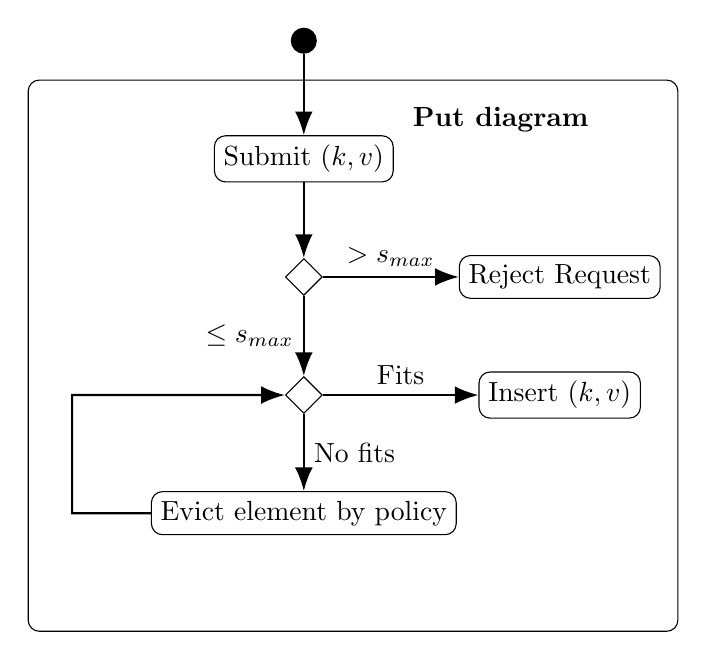
\begin{tikzpicture}[node distance=1.5cm]
        % Frame
        \draw [rounded corners] (-3.5,-1.5) rectangle (4.75, -8.5);
        \node (title) at (2.5, -2) {\textbf{Put diagram}};
        
        % Nodes
        \node[initial] (initial) at (0,-1) {};
        \node[action, below of = initial] (submit)  {Submit $(k, v)$};
        \node[decision, below of = submit] (maxCapacityDecision)  {};
        \node[action, right of = maxCapacityDecision, xshift=1.75 cm] (reject) {Reject Request};
        \node[decision, below of = maxCapacityDecision] (fitsDecision) {};
        \node[action, right of = fitsDecision, xshift=1.75 cm](insert){Insert $(k, v)$};
        \node[action, below of = fitsDecision](evict){Evict element by policy};
        \draw [arrow] (initial) -- (submit);
        \draw [arrow] (submit) -- (maxCapacityDecision);
        \draw [arrow] (maxCapacityDecision) -- (reject)node[midway, above]{$> s_{max}$};
        \draw [arrow] (maxCapacityDecision) -- (fitsDecision) node[midway, left]{$\leq s_{max}$};
        \draw [arrow] (fitsDecision) -- (insert) node[midway, above]{Fits};
        \draw [arrow] (fitsDecision) -- (evict) node[midway, right]{No fits};
        \draw [arrow] (evict.west) -- ++(-1cm, 0) -- ++(0, 1.5) -- (fitsDecision.west);
    \end{tikzpicture}
    \caption{Activity diagram for general put showing eviction.}
    \label{fig:general_put_workflow}
\end{figure}

\subsubsection{Persistency}
One main goal of this project is to have a cache that is \textit{persistent}.
We define persistency as the ability to recover the cache
after a crash or a power failure. In practice, this means the following.
Let $D$ and $DB$ be the directory and SQLite database used to initialize
the cache $X$. Assuming we store $(k, v)$ into $X$ and the program crashes,
it possible to initialize a new instance $X'$ of the same cache $X$ using the same
directory $D$ and database $DB$. Then, doing $X'.get(k)$ should return $v$.

\begin{tcolorbox}[colback=blue!5!white, colframe=blue!75!black, title=Note]
    It is theoretically possible to have two caches $X$ and $Y$ pointing
    to the same persistency $D$ and $DB$. However, this is not recommended
    because \sqlitecache~is a single-threaded cache.
\end{tcolorbox}

\subsubsection{Settings \& Recovery}
Assume that you want to reconnect to a cache $X$ that was previously
created using the same directory $D$ and database $DB$. To do so, you can
create a new instance $X'$ using the same directory and database.

Recall that our cache has three possible settings: maximum size, encryption, and compression.

The cache $X'$ will automatically detect these settings and use them. As a result,
if a developer creates $X'$ using a different set of settings, the cache will
ignore and override them in favor of the settings stored in disk.
All settings are unique and stored
in the metadata table $(M)$. This behavior is enforced by the UNIQUE
constraint in the metadata table $(M)$ and inserting
settings using the \texttt{ON CONFLICT DO NOTHING} clause.

%% LRUCache subsection
\subsection{LRUCache\label{sec:lru}}
The schema used for the cache table $C$ used by the LRUCache
is given by \autoref{fig:lru_cachetable_relation}. We track
recency by using the \texttt{accessed\_at} attribute. There
are not triggers that automatically update this value. Instead,
we update this value for every call to the \texttt{get(k)}
method.

During eviction, we sort the values
by the access time and evict enough items
such that a new $(k, v)$ pair can be inserted.

\begin{figure}[!htp]
    \centering
    \begin{tikzpicture}
        \umlclass[type=class]{LRUPrimaryCache}{
            key : INTEGER \\
            filename : TEXT \\
            size : INTEGER \\
            stored\_at : TIMESTAMP \\
            accessed\_at : INTEGER
        }{}
    \end{tikzpicture}
    \caption{UML class diagram for the LRUPrimaryCache relation.}
    \label{fig:lru_cachetable_relation}
\end{figure}

% LFUCache subsection
\subsection{LFUCache\label{sec:lfu}}
The schema use for the cache table $C$ is
described in \autoref{fig:lru_cachetable_relation}.
Note that we use the \texttt{accessed\_count} attribute
in $C$ to track how many times a particular key
has been accessed. However, LFUCache supports two eviction
policies: ttl based and accessed count based.

In count based eviction,
we sort the elements by their access count and
start evicting them until enough space is created
such that a new value $v$ fits into the cache.
We do not use triggers to update access counts. Instead,
we manually increment the counter whenever a key is requested.
We consider a request any moment \texttt{get(k)} is invoked.

In ttl based eviction,
we recompute the a new ttl by
\[
ttl_{new} = ttl - (now - stored\_at)
\]
where $now$ is the current timestamp of the system.
After recomputing the new ttl, we sort the $(k, v)$
pairs until enough space becomes available to insert a new $v'$.

It is important to note that we handle expired $(k, v)$ pairs
on demand. This means that there is no background process
constantly evicting expired elements. We perform
a cleanup of expired data whenever data is requested
from the cache by using ~\texttt{get(k)}. Additionally,
we perform cleanup whenever eviction needs to take place.

\begin{figure}[!htp]
    \centering
    \begin{tikzpicture}
        \umlclass[type=class]{LFUPrimaryCache}{
            key : INTEGER \\
            filename : TEXT \\
            size : INTEGER \\
            stored\_at : TIMESTAMP \\
            accessed\_count : INTEGER \\
            ttl : REAL
        }{}
    \end{tikzpicture}
    \caption{UML class diagram for the LFUPrimaryCache relation.}
    \label{fig:lfu_cachetable_relation}
\end{figure}


% Subsection to discuss the hybrid cache.
\subsection{HybridCache\label{sec:hybrid}}
Our HybridCache uses the eviction 
policy defined in~\cite{shah2023ImprovedCacheEviction}.
Internally, this cache uses a combination of an LRUCache and a
LFUCache with TTL. Let $P, Q$ be the capacity
of the underlying LRUCache and LFUCache objects.
At any point in time, elements are stored in only
one of the caches. Elements are initially placed
into the LRUCache and they are eventually moved
from LRUCache into the LFUCache after a particular
access threshold is reached.

Formally,
let a HybridCache define a threshold $T$, 
a default TTL $\tau$, and a counter $\hybridCounter$. Every time a
value $v$ for $k$ is looked up into the cache,
we increment $\hybridCounter[k]$. We move
the entire $(k, v)$ pair
from LRUCache into LFUCache 
whenever $\hybridCounter[k] > T$
with TTL $\tau$.
Recall that eviction policies trigger automatically
on insertions. Therefore, moving
an element into the LFUCache \textbf{does not}
bypass the eviction workflow defined in \autoref{fig:put_sequence_diagram}.

Note that when getting a value $v$ for $k$,
we perform a lookup in both LRUCache and LFUCache
to know where it exists. Given that LFUCache with TTL
evicts on demand, this lookup will trigger eviction
of expired elements \textemdash~guaranteeing
correctness.

%% DiskStorage subsection
\subsection{DiskStorage}
DiskStorage is a python class responsible for managing a given directory $dir$.
Under the hood, the values $v$ are stored in different files
under $dir$. Because its responsibility is to handle values,
all value oriented operations such as compression/decompression,
encryption/encryption are provided as methods on this class.

The primary motivation of having the value storage decoupled
from the primary cache in the SQLite database is the possibility
of extending value storage using a different protocol for serialization,
such as JSON.

%% Testing subsection
\subsection{Testing}
All the functionality of the \sqlitecache~package is \textbf{functionally} tested using
the \texttt{pytest} framework. The tests are located inside the \texttt{tests} directory.

We selected the pytest framework because it is the most popular testing framework
for Python. Furthermore, the isolation and lifecycle of the tests and fixtures
are well defined. This allows us to have a clean and isolated environment
for each test. Finally, any long-running tests,
such as tests for TTL based policies and simulation tests,
are marked as \textit{slow}. Refer
to \autoref{fig:testing_running} for a
screenshot of a test session.

\begin{figure}[!htp]
    \centering
    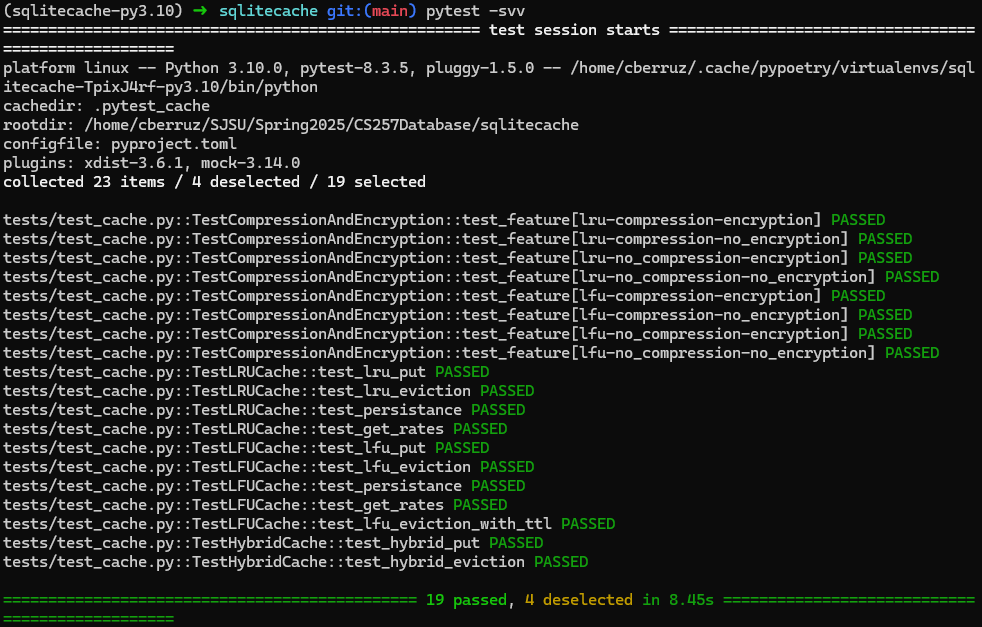
\includegraphics[width=\columnwidth]{images/testing.png} 
    \caption{Testing using pytest.}
    \label{fig:testing_running}
\end{figure}

%% Simulation Subsection
\subsection{Simulation\label{sec:simulation}}
The following section describes in detail the simulation, focusing on the differences
between our methodology and the methodology used in~\cite{shah2023ImprovedCacheEviction}.

The first difference is that our cache is persistent.
The authors in~\cite{shah2023ImprovedCacheEviction} rely on the assumption
that retrieval of elements and count tracking is \textit{efficient}. Given
that they used a memory-based cache and that there was no strict definition
of efficiency, our results are expected to not be identical.

The second difference is that our cache is a key-value cache instead
of an element-oriented cache. The main difference is the hash computation.
In an element-oriented cache, the hash is computed over the element itself
while in our key-value cache, the hash is computed over the key.
As a result, instead of creating 500 unique python objects,
we create 500 unique (key, value) string pairs instead. See
\autoref{eq:experiment_value_set} for more details
\begin{equation}
D = \{(k, v) \mid k = v, k = \{\text{`001'}, \text{`002'}, \ldots, \text{`500'}\}\}
\label{eq:experiment_value_set}
\end{equation}

The third difference is the concept of \textit{size}.
Cache size in~\cite{shah2023ImprovedCacheEviction}
is count based. For example, if a cache has capacity of a 100,
this means that the cache can hold up to 100 elements of
arbitrary size. As a result, let $P$ be the count capacity
of a count-sized cache. In order to find our equivalent byte-sized
cache, we can let all values be of homogenous size $b$.
Then, the byte-sized capacity $(P')$ for our cache, as defined
in~\ref{sec:size_description}, is simply
\begin{equation}
    P' = P \times b
    \label{eq:byte_capacity}
\end{equation}
Note that~\autoref{eq:experiment_value_set} defines $D$ is such a way
that~\autoref{eq:byte_capacity} holds true for our experimentation
as all values are strings of length 3.

The fourth difference is how misses are handled.
It is not clear why the
authors in~\cite{shah2023ImprovedCacheEviction}
automatically insert an element when it is missing.
A simple example of how a cache
is generally used is provided in \autoref{fig:cache_example}.

% python cache code example
\begin{figure}[ht]
    \centering
    \begin{tcolorbox}[colback=gray!5!white, colframe=gray!75!black, title=General Cache Example]
    \begin{verbatim}
if cache.get("key") is None:
    value = expensive_op()
    cache.put("key", value)
return cache.get("key")
    \end{verbatim}
    \end{tcolorbox}
    \caption{Example of cache usage in Python.}
    \label{fig:cache_example}
\end{figure}

Although \autoref{fig:cache_example}
represents a Python code snippet, the same
applies for other scenarios. For example,
a database stores pages in the buffer. When a
page fault
occurs, the database performs an I/O, which
is expensive, to retrieve the page.
Therefore, we did not include automatic
insertion of an element into the cache, in
the event of a miss, at the cache classes level.

However, during simulation, we do automatic insertion
during misses. Recall that during simulation
all our (key, value) pairs have form $(k, k)$
drawn from $D$.
Therefore, if \texttt{get(k)} returns \texttt{None},
we can insert a new pair by calling \texttt{put(k, k)}.
This change makes it possible to run our simulation
as close as possible to~\cite{shah2023ImprovedCacheEviction}.

The final difference is the hit and miss rates tracking mechanism.
All of our cache classes keep up-to-date hit and miss
rate statistics. This is done internally, with an I/O overhead.
Given that the HybridCache uses the TTL feature
of the LFUCache, \textit{runtime} has a direct
impact. To reduce the I/O overhead
of retrieving the hit and miss rates from
the cache, we use an auxiliary in-memory hash map.
For a concise version of the simulation,
refer to Algorithm~\ref{alg:simulation}.

\begin{algorithm}
    \caption{Simulation for any given Cache}
    \label{alg:simulation}
    \begin{algorithmic}[1]
    \Require Cache $C$; Dataset $D = \{(k, v) \mid k = v, k \in \{\text{`001'}, \text{`002'}, \ldots, \text{`500'}\}\}$
    \Require $P=100$, value size $b$, and Cache capacity $P'$
    \Require $N$ total requests,
        in-memory tracking hashmap $H$
    \For{$i = 1$ to $N$}
        \State Randomly select $(k, v)$ from $D$
        \State $value \gets \text{C.get}(k)$
        \If{$value = \text{None}$}
            \State $\text{C.put}(k, v)$
        \EndIf
        \State Push hit rate, miss rate, $i$ into $H$.
    \EndFor
    \end{algorithmic}
\end{algorithm}

\section{Results and Discussion}
% Describe evaluation methodology and significant results in the evaluation section
% Evaluate the selected approach and analyze why the selected approach is good?
%   Provide an intuitive description of the algorithms, their correctness and their complexity
The simulation was run
on a Dell Laptop with a 11th Gen Intel(R) Core(TM) i7-11800H processor (8 cores, 16 threads)
running at 2.30GHz, 64.0 GB of installed RAM,
a 64-bit operating system with an x64-based processor
using Python3.10 and pytest as the driver.
We selected Pytest because the test-isolation generalizes
well for simulations. Therefore, simulations
are `tests' marked with the \texttt{@pytest.mark.simulation}
marker. Because running a simulation is slow,
these tests are also marked as \textit{slow}.
More importantly, we run our simulation
distributed across multiple CPUs. Given that
each simulation is isolated, we can run
all the simulations in parallel
by using pytest-xdist framework~\cite{pytestXdist}.
Additionally, pytest ships with runtime
tracking out of the box.
Refer to \autoref{fig:simulation}
for an example output of a running simulation.

\begin{figure}[!htp]
    \centering
    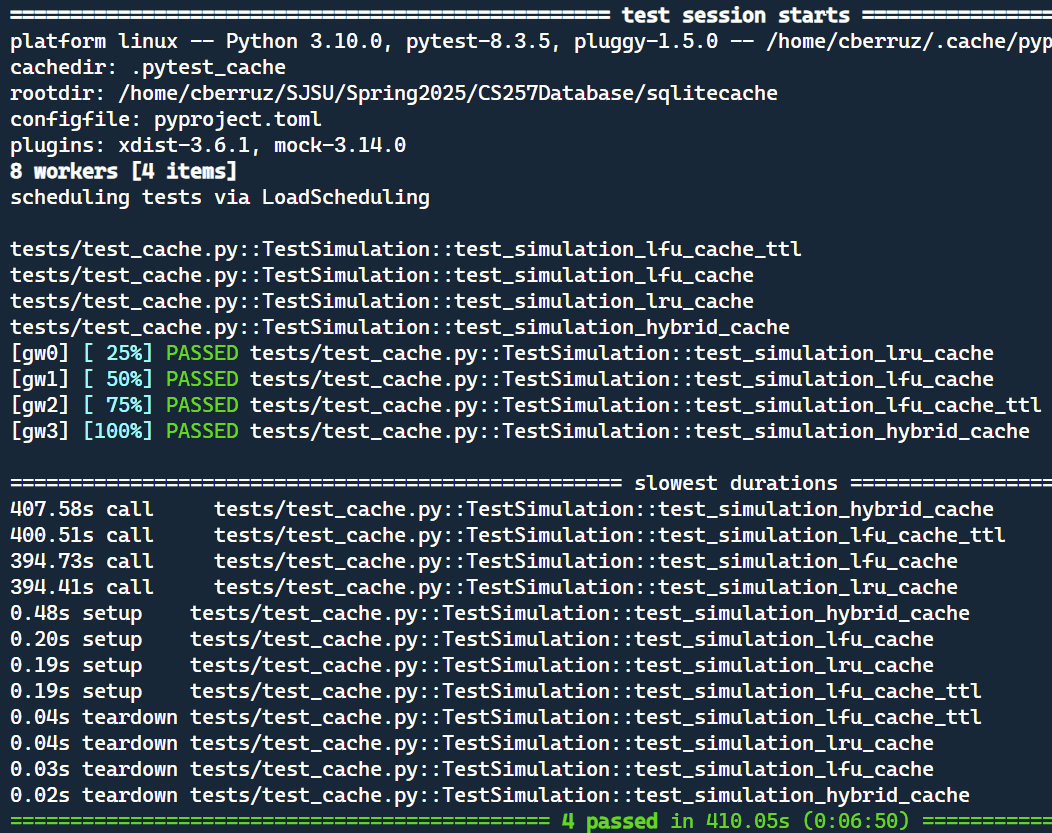
\includegraphics[width=\linewidth]{images/simulation_running_example.png}
    \caption{Screenshot of a running simulation.}
    \label{fig:simulation}
\end{figure}

We let $P = 100$.
In our platform, all uncompressed and unencrypted
values in $D$ occupy $b = 18$ bytes.
Therefore, the cache size $P' = Q' = 1800$ bytes.
Furthermore, no compression and no encryption
was enabled.

The simulation was run as a sustained load,
as described in Algorithm~\ref{alg:simulation}.
This means that it runs until completion
for
$N$ requests. For example, in $N=1000$
we generate 1000 data points for both
the hit and miss rates. The duration
of each simulation run was dependent
on the eviction policy being tested.
TTL based policies, such as LFUCacheTTL
and HybridCache as seen in \autoref{fig:simulation}.

\begin{figure*}[!htp]
    \centering
    \begin{tikzpicture}
        \begin{axis}[
            width=\linewidth*0.9,
            height=8cm,
            xlabel={n\_requests},
            ylabel={hit\_rate},
            grid=major,
            legend style={at={(0.95,0.05)}, anchor=south east},
            title={Hit Rate vs. Number of Requests}
        ]
        \addplot[
            color=blue,
        ] table [
            col sep=comma,
            x={requests},
            y={hit_rate}
        ] {data/LRUCacheSimulationResults.csv};
        \addplot[
            color=red,
        ] table [
            col sep=comma,
            x={requests},
            y={hit_rate}
        ] {data/LFUCacheSimulationResults.csv};
        \addplot[
            color=orange,
        ] table [
            col sep=comma,
            x={requests},
            y={hit_rate}
        ] {data/LFUCacheTTLSimulationResults.csv};
        \addplot[
            color=black,
        ] table [
            col sep=comma,
            x={requests},
            y={hit_rate}
        ] {data/HybridCacheSimulationResults.csv};
        \legend{LRUCache, LFUCache, LFUCacheTTL, HybridCache}
        \end{axis}
    \end{tikzpicture}
    \caption{Hit rate as a function of number of requests for different cache eviction policies.}
    \label{fig:hit_rate_plot}
\end{figure*}

A total of four eviction policies were tested:
LRU, LFU, LFU with TTL, and Hybrid.
The results of the hit rate vs. the number
of request for each eviction policy is summarized
in \autoref{fig:hit_rate_plot}.

It is clear that the HybridCache policy performs significantly
better than all other policies. The LRUCache performs the worst
among all eviction policies. These results
are in alignment with~\cite{shah2023ImprovedCacheEviction}.

\section{Conclusion}
% Conclusions, lessons learned possible improvements, etc.
Summarize your findings and suggest future work.

\bibliographystyle{IEEEtran}
\bibliography{references}

\end{document}